\documentclass[a4paper,12pt]{article}
\addtolength{\oddsidemargin}{-1.cm}
\addtolength{\textwidth}{2cm}
\addtolength{\topmargin}{-3cm}
\addtolength{\textheight}{3.5cm}
\makeindex


\usepackage[pdftex]{graphicx}
\usepackage{makeidx}
\usepackage{float}
\usepackage{hyperref}
\hypersetup{
	colorlinks=true,
	linkcolor=blue,
	filecolor=magenta,      
	urlcolor=cyan,
}


% define the title
\author{Team Delta}
\title{ Assignment 1}
\begin{document}
	\setlength{\parskip}{6pt}
	
	% generates the title
	\begin{titlepage}
		\begin{center}
			
\includegraphics[width=1\textwidth]{./Pictures/up_logo.png}\\[1.5cm] 
			\textsc{\LARGE Department of Computer Science} \\ [.5cm]
			\textsc{\Large Tender} \\ [.5cm]
			\textsc{\Large Project: DropOff} \\ [.5cm]
			\line(1,0){450}\\[.5cm]
			\huge{\bfseries Client: Gavin Potgieter}\\
			\line(1,0){450}\\[.5cm]
			\textsc{\LARGE Team: CodeBlox}\\ [0.5cm]
			
			
			\textsc{\large Tshepo Malesela (Bsc: Computer Science)}\\
			\textsc{\large Lethabo Mogase (Bsc: Computer Science)}\\
			\textsc{\large Lorenzo Spazzoli (Bsc: Computer Science)}\\
			\textsc{\large Bilal Muhammad (BIS: Multimedia)}\\
			\textsc{\large Dirk de Klerk (BIS: Multimedia)}\\ [3.9cm]
			
			\large\today
		\end{center}
	\end{titlepage}
	
	\tableofcontents
	\thispagestyle{empty}
	\footnotesize
	\normalsize
	
	
	
	
	\newpage
	\section{The Team}
	
	\includegraphics[width=1\textwidth]{./Pictures/the_group.jpg}\\
	
	{\noindent}Each team member possesses a wide variety of skill sets and characteristics that will ultimately contribute to the success of this project. All of our members work well together and are diligent in their work. We as a team take deadlines rather seriously and strive to deliver high quality work well before final submission dates.  
	
		\newpage
		\subsection{Tshepo Malesela}
		\includegraphics[width=1\textwidth]{./Pictures/the_group.jpg}\\
			\subsubsection{Interests}
			As a computer science student, my interests have changed over the past three years. Ive always had a profound deep interest in computing, I had no one to introduce me to programming as there was no one at home who worked in such an industry or knew anything about it. A lot of interests have changed over the past three years but my love for discovery and knowledge hasn't.
			
			\subsubsection{Technical Skills}
			I only started my computer learning properly in  my first year, it was difficult to adjust to so much information being thrown at me but over some time I began enjoying it, I gained skills in Object Oriented languages such as  as C++, C, Java, scripting languages such as javascript and php, and lastly some special-purpose languages such as php. I understand these languages well, studying computer science mens you also need to do more than just school work, so I started reading books and writing programs in my spare time.
			
			\subsubsection{Past Experiences}
			For one of our courses (Software Engineering), we where introduced to so many technologies and also had to use them to complete a project. I believe the knowledge we were introduced to will aid me in adding valuable input to this project.
			
			\subsubsection{Non-technical Strengths}
			I am open to new things, I love experiencing things I'm not familiar with as well. I'm also a very fair person. I am also disciplined. I communicate well with others and this wil hep because I am working in a group.
			\subsubsection{My motivation for wanting to do this project}
			I have a very strong and passionate interest for technology. I really enjoy finding out how different technologies works and picture how I can use it or  how it is used in the real world. I also enjoy making things work better. I know that I will be fully dedicated to this project because I interests me in the deepest way, I really believe that my group and I will enjoy developing this for you and I have no doubt that it will be done to the greatest of our abilities.  
		
		\newpage
		\subsection{Lethabo Mogase}
		\includegraphics[width=1\textwidth]{./Pictures/the_group.jpg}\\
			\subsubsection{Interests}
			
			\subsubsection{Technical Skills}
			
			\subsubsection{Past Experiences}
			
			\subsubsection{Non-technical Strengths}
			
			\subsubsection{My motivation for wanting to do this project}
		
		\newpage
		\subsection{Lorenzo Spazzoli}
		\includegraphics[width=1\textwidth]{./Pictures/the_group.jpg}\\
			\subsubsection{Interests}
			
			\subsubsection{Technical Skills}
			
			\subsubsection{Past Experiences}
			
			\subsubsection{Non-technical Strengths}
			
			\subsubsection{My motivation for wanting to do this project}
		
		\newpage
		\subsection{Bilal Muhammad}
		
\includegraphics[scale=0.2]{./Pictures/bilal.jpg}\\
			\subsubsection{Interests}
			I have always been passionate about programming and creating innovative technology that has not been seen before. I enjoy playing cricket, singing and cooking. But most of all I like experimenting with different viruses and finding ways to break code.
			\subsubsection{Technical Skills}
			I am equipped with the knowledge of the following languages and technologies - C++, Java (EE), PHP, JavaScript, HTML and CSS, Assembly x64 and MySql/PostGres.
			\subsubsection{Past Experiences}
			I am currently working for the CS department as a tutor for a C++ module, where I create assignments and memos. I was also part of the Integration(High level) team for the Mini Project that we successfully completed this year. I am also currently doing a networking course which I think will be helpful for this project  
			\subsubsection{Non-technical Strengths}
			I have always been a strong candidate for leadership positions, mainly because I am understanding and can find reasonable solutions easily. My communication skills are solid which makes me a strong team player.
			\subsubsection{My motivation for wanting to do this project}
			This is my passion - creating innovative technology. "The difference between the impossible and the possible lies in a person's determination."
		
		\newpage
		\subsection{Dirk de Klerk}
		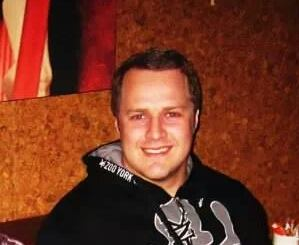
\includegraphics[scale=0.8]{./Pictures/dirk.jpg}\\
			\subsubsection{Interests}
			I have a great fondness for music and practice the electric guitar when I get the chance. I also enjoy exercise, cooking, and spending time with family and friends.
			\subsubsection{Technical Skills}
			I consider myself to be a descent programmer, I also have an eye for aesthetic design. Languages include: Java, C++, Javascript, PHP, Assembler64, XML, SQL, and HTML. 
			\subsubsection{Past Experiences}
			I gained some experience during the mini-project of Software Engineering, where I was part of the integration team. This gave me good exposure to the Java ecosystem as well as a basic understanding of how layered systems work.
			\subsubsection{Non-technical Strengths}
			I am a very ambitious person, that works very diligently, paying close attention to details. I also consider myself to be a natural leader and work well in teams. 
			\subsubsection{My motivation for wanting to do this project}
			My main interest in this particular project, is the technologies that I will get to work with. I am always looking to challenge myself and discover new ideas.
	\newpage
	\section{Project Execution}
	
	\subsection{Development Methodology}  
	
	The Methodology that will be used in this project is the Agile Development Process. We as a group feel like this methodology will be the most failure and fault proof way to go. In this methodology, we intend to follow the Spiral process because in this way we can adopt elements from other process models such as waterfall, incremental and evolutionary prototyping.

	{\noindent}As a group we decided on the spiral process model because in this project decisions will be made on how to implement the functionality and architecture. With the spiral process model we will choose the safest options that will yield the best results. There is high risk analysis with this process model, and it is the preferred choice for many large and mission critical projects, therefore it will suit our project well.

	{\noindent}The spiral process model also has great features such as the ability to add extra functionality at a later stage in the project. This will probably be the case as the project progresses.

	
	\newpage
	\subsection{Developer/Client Communication}
	
	\newpage
	\subsection{Technical Challenges}
	
	\newpage
	\subsection{Technology Stack}
	
	\newpage
	\subsection{Deliverables}
	
	
	\newpage
	\section{Conclusion}
	
	Should you require any further information, feel free to contact our team lead, Bilal Muhammad on:
	
	\begin{itemize}
		\item[$\bullet$]Cell: 072 878 7807
		\item[$\bullet$]Email: bilibongers@gmail.com
	\end{itemize}
	We are extremely excited to be working on this project and also look forward to be working with you.
	
	
\end{document}
